\documentclass[cn,table]{elegantbook}

\usepackage{tikz}
\usepackage{graphicx}
\usepackage{subcaption}
\usepackage[ruled,linesnumbered,vlined]{algorithm2e}
\usepackage{hyperref}
\usepackage{listings}
\usepackage{interval}
\usepackage{xcolor}
\usepackage{ulem}
\usepackage{wrapfig}

\intervalconfig{%
	soft open fences,
}

\def\figureautorefname{图}
\def\sectionautorefname{小节}

\SetAlgorithmName{算法}{算法}{算法索引}

\renewcommand*{\lstlistingname}{代码}

\title{何老师算法课笔记}
\subtitle{Always be patient, sharp and diligent.}
\author{计卓1801全体}
\institute{华中科技大学}
\date{\zhtoday}
\version{2.0.0}
\logo{logo.png}
\cover{cover.png}

\begin{document}
\maketitle
\tableofcontents
\pagenumbering{arabic}

% add your code here
% \input{src/example.tex}
\input{src/Ln1-AsymptoticOrderGrowth.tex}
\input{src/Tiling-Problem.tex}
\input{src/stable-matching.tex}
\input{src/Greedy-algorithm.tex}
\input{src/Ln06-MST.tex}
\input{src/Ln07-redblue.tex}
\input{src/Ln9-NearestPoints.tex}
\chapter{主定理(主方法)}
\begin{introduction}
	\item 主定理的内容
	\item 主定理的用途
	\item 主定理的证明
\end{introduction}
\section{主定理的内容}
已知$T(n) = a T(\frac{n}{b}) + f(n)$,其中$a\geq 1, b\geq 1, f(n)$已知,则:
$$
\begin{array}{l}  
  \left\{\begin{matrix} 
  f(n) = O(n^{\log_{b}{a} - \epsilon} ),~T(n) = \Theta(n^{\log_{b}{a}} )  \\ 
  f(n) =  \Theta(n^{\log_{b}{a}} ),~T(n) = \Theta(n^{\log_{b}{a}}\log_{}{n} ) \\ 
  f(n) = \Omega (n^{\log_{b}{a} + \epsilon} ),T(n) = \Theta (f(n))
\end{matrix}\right.    
\end{array} 
$$
\section{主定理的用途}
        \begin{figure}[h]
	\begin{minipage}[t]{1\linewidth}
		\centering
		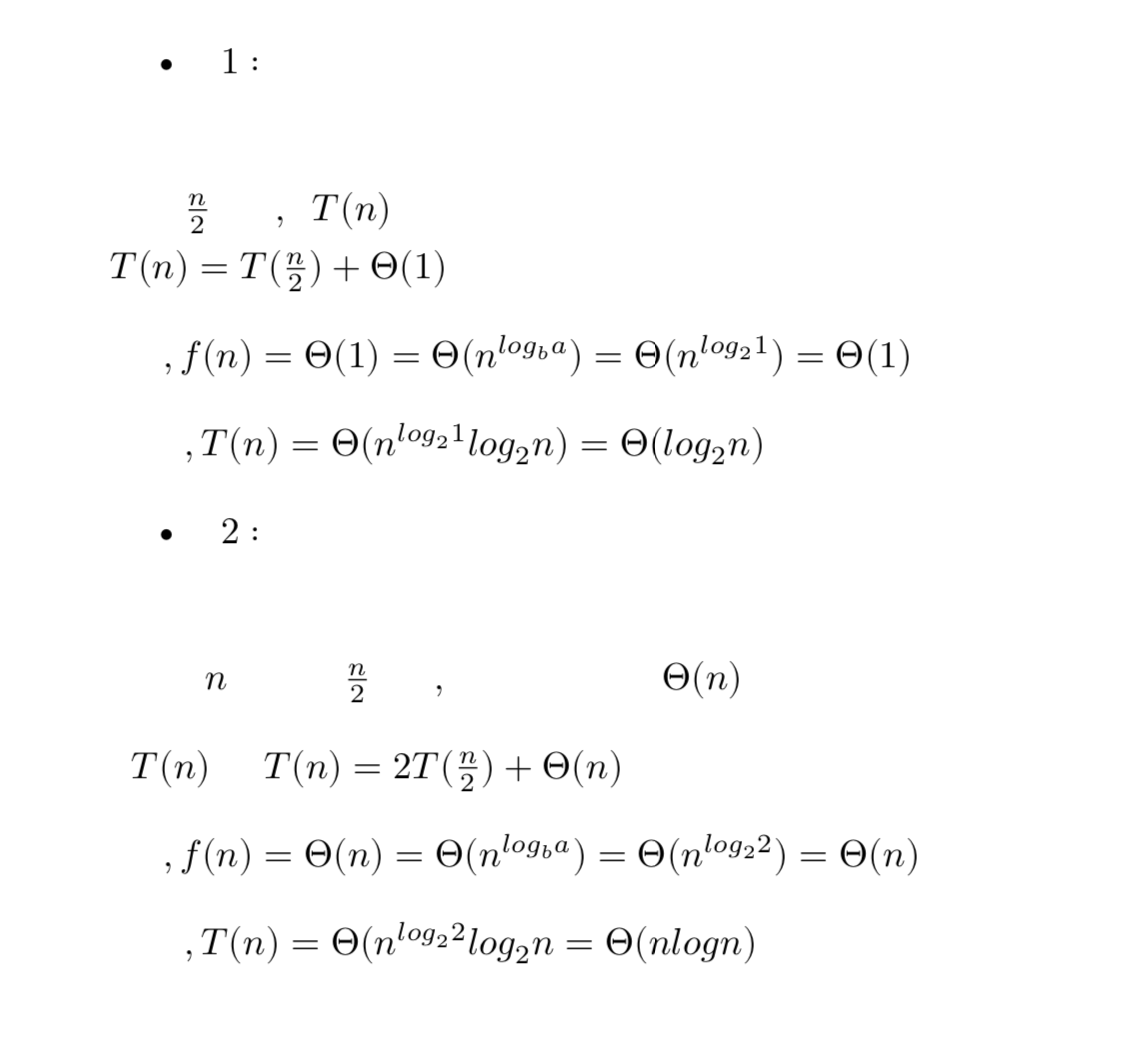
\includegraphics[width=10cm,height=5cm]{image/main1.png}
	\end{minipage}
\end{figure}
\section{主定理的证明}
\begin{figure}[h]
	\begin{minipage}[t]{1\linewidth}
		\centering
		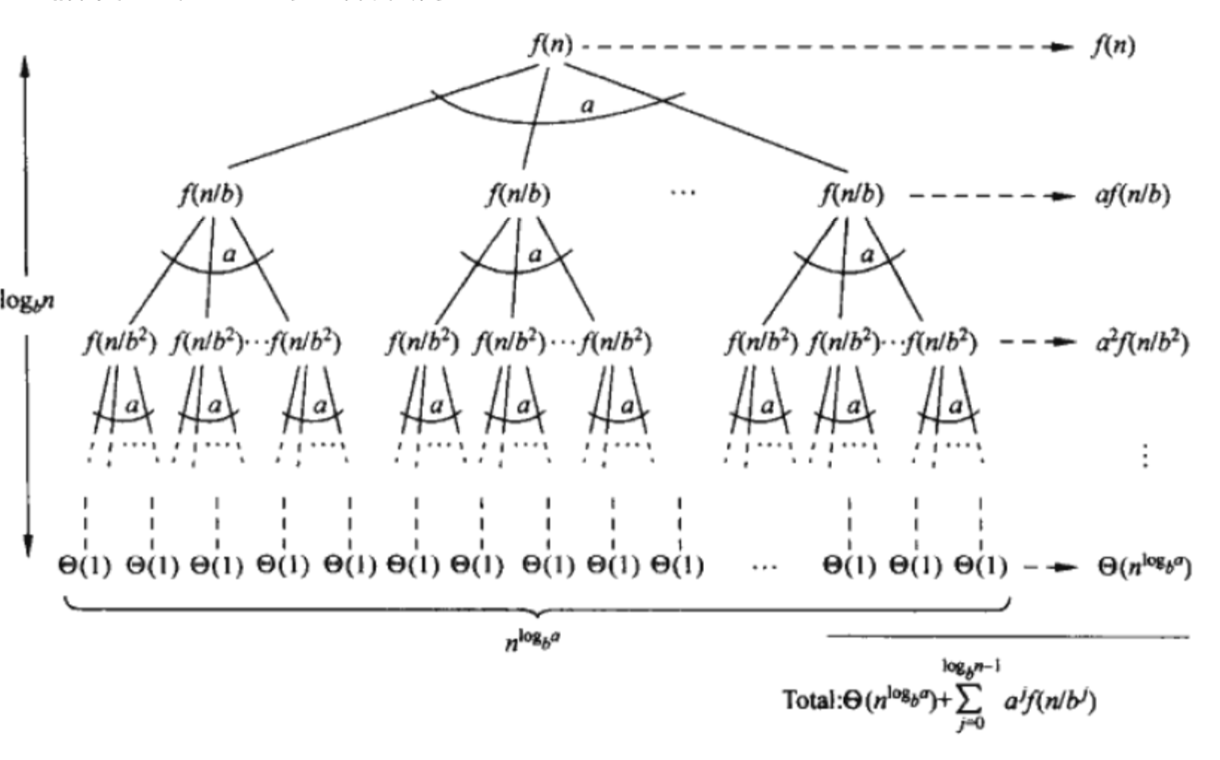
\includegraphics[width=10cm,height=3.5cm]{image/mainmaster.png}
		\caption{递推式展开}
	\end{minipage}
\end{figure}
\subsection{假设 n 是 b 的整数次方}
$T(n)=\Theta\left(n^{\log _{a} b}\right)+\sum_{j=0}^{\log _{b} n-1} a_{j} f\left(n / b^{j}\right)$\\
(1)
 $$
 \begin{array}{l}
f(n)=O\left(n^{l o g_{b} a-\epsilon}\right) \\
g(n)=\sum_{j=0}^{\log _{b} n-1} a_{j} f\left(n / b^{j}\right) \\
f\left(n / b^{j}\right)=O\left(\left(\frac{n}{b^{j}}\right)^{\log _{b} a-\epsilon}\right) \\
c, n_{0}, \forall n \geq n_{0} \\
\left.f\left(n / b^{j}\right) \leq c\left(\frac{n}{b^{j}}\right)^{l o g_{b} a-\epsilon}\right) \Rightarrow a^{j} f\left(n / b^{j}\right) \leq c a^{j}\left(\frac{n}{b^{j}}\right)^{\log _{b} a-\epsilon} \\
a^{j} f\left(n / b^{j}\right) \leq c n^{\log _{b} a-\epsilon}\left(\frac{a}{b^{\log _{b} a-\epsilon}}\right)^{j} \\
\Rightarrow a^{j} f\left(n / b^{j}\right) \leq c n^{\log _{b} a-\epsilon}\left(\frac{a b^{\epsilon}}{b^{\log _{b} a}}\right)^{j} \\
\Rightarrow a^{j} f\left(n / b^{j}\right) \leq c n^{\log _{b} a-\epsilon}\left(b^{\epsilon}\right)^{j} \\
g(n) \leq c n^{\log _{b} a-\epsilon} \sum_{j=0}^{\log _{b} a-1}\left(b^{\epsilon}\right)^{j} \\
\Rightarrow \\g(n) \leq c n^{\log _{b} a-\epsilon} \frac{1\left(1-\left(b^{\epsilon}\right)^{l o g_{b} n}\right)}{1-b^{\epsilon}}
\Rightarrow g(n) \leq c n^{\log _{b} a-\epsilon \frac{1-n^{\epsilon}}{1-b^{\epsilon}}} \\
\Rightarrow g(n) \leq c \frac{n^{\log _{b} a-\epsilon}-n^{\log _{b} a}}{1-b^{\epsilon}} \\
g(n)=O\left(n^{\log _{b} a}\right) \\
T(n)=\Theta\left(n^{\log _{b} a}\right)+O\left(n^{\log _{b} a}\right)=\Theta\left(n^{\log _{b} a}\right)
\end{array}
 $$
(2)
$$
\begin{array}{l}
f(n)=\Theta\left(n^{\log _{b} a}\right) \\
g(n)=\sum_{j=0}^{\log _{b} n-1} a_{j} f\left(n / b^{j}\right) \\
f\left(n / b^{j}\right)=\Theta\left(\left(\frac{n}{b^{j}}\right)^{\log _{b} a}\right) \\
c_{1}, c_{2}, n_{0}, \forall n \geq n_{0} \\
c_{1}\left(\frac{n}{b^{j}}\right)^{l o g_{b} a} \leq f\left(n / b^{j}\right) \leq c_{2}\left(\frac{n}{b^{j}}\right)^{l o g_{b} a} \Rightarrow c_{1} a^{j}\left(\frac{n}{b^{j}}\right)^{l o g_{b} a} \leq a^{j} f\left(n / b^{j}\right) \leq c_{2} a^{j}\left(\frac{n}{b^{j}}\right)^{\log _{b} a} \\
c_{1} n^{\log _{b} a}\left(\frac{a}{b^{\log _{b} a}}\right)^{j} \leq a^{j} f\left(n / b^{j}\right) \leq c_{2} n^{\log _{b} a}\left(\frac{a}{b^{\log _{b} a}}\right)^{j} \\
\Rightarrow c_{1} n^{\log _{b} a} \leq a^{j} f\left(n / b^{j}\right) \leq c_{2} n^{\log _{b} a} \\
\Rightarrow c_{1} n^{\log _{b} a} \lg n \leq g(n) \leq c_{2} n^{\log _{b} a} \lg n \\
g(n)=\Theta\left(n^{\log _{b} a} \lg n\right)
\end{array}
$$
(3)

$$
\begin{array}{l}
f(n)=\Omega\left(n^{\log _{b} a+\epsilon}\right) \\
c<1 \text { af }\left(\frac{n}{b}\right) \leq c f(n) \\
g(n)=\sum_{j=0}^{\log _{b} n-1} a^{j} f\left(\frac{n}{b^{j}}\right) \\
a f\left(\frac{n}{b}\right) \leq c f(n) \\
\Rightarrow a^{j} f\left(\frac{n}{b^{j}}\right) \leq c^{j} f(n) \\
\Rightarrow g(n) \leq \sum_{j=0}^{\log _{b} n-1} c^{j} f(n) \\
\Rightarrow g(n) \leq \sum_{j=0}^{+\infty} c^{j} f(n)\\
\Rightarrow g(n) \leq \frac{1}{1-c} f(n) \\
g(n)=O(f(n))
\end{array}
$$

\subsection{假设 n 不是 b 的整数次方}
$T(n)=a T\left(\left\lfloor\frac{n}{b^{j}}\right\rfloor\right)+f(n) T(n)=a T\left(\left\lceil\frac{n}{b}\right\rceil\right)+f(n)$

$$
\begin{array}{c}
a^{\left\lfloor\log _{b} n\right\rfloor}<a^{\log _{b} n}<a * a^{\left\lfloor\log _{b} n\right\rfloor}, \\\quad \Theta\left(a^{\left\lfloor\log _{b} n\right\rfloor}\right)=\Theta\left(a^{\log _{b} n}\right)\\T(n)= 
\Theta\left(a^{\left\lfloor\log _{b} n\right\rfloor}\right)+\sum_{j=0}^{\left\lfloor\log _{b} n\right\rfloor-1} a^{j} f\left(n_{j}\right)\left(n_{j}=\left\lceil\frac{n}{b^{j}}\right\rceil\right) \\
\cdot \frac{n}{b^{j}} \leq \quad\left[\frac{n}{b^{j}}\right\rceil \quad<\quad \frac{n}{b^{j}}+1\\ \quad  \quad  \left\lceil\frac{n}{b^{j}}\right\rceil\left(\Theta\left(\frac{n}{b^{j}}\right)=\right. 
\left.\Theta\left(\left\lceil\frac{n}{b^{j}}\right\rceil\right)\right) 
\end{array}
$$



\input{src/Ln11-LargeIntegerMultiplication.tex}
\chapter{分治算法之矩阵乘法}
\begin{introduction}
	\item 问题引入
	\item 用分治法解决
\end{introduction}
\section{问题引入}
在线性代数中我们学习过矩阵乘法,已知规模为 $n$ 的矩阵 $A$ 和 $B$,我们可以直接计算行列积算法的复杂度,单次数乘的复杂度我们已知是$ O(1)$每次计算行列积需要进行$n$次乘法,总共需要计算$n^2$次行列积,所以不难得知基于行列积的矩阵乘法复杂度为$O(n^3)$
如果我们尝试分治策略,结果会怎么样呢?首先我们将矩阵$C = AB$进行二分。
$$
A=\left[\begin{array}{ll}
A_{11} & A_{12} \\
A_{21} & A_{22}
\end{array}\right] B=\left[\begin{array}{ll}
B_{11} & B_{12} \\
B_{21} & B_{22}
\end{array}\right] C=\left[\begin{array}{ll}
C_{11} & C_{12} \\
C_{21} & C_{22}
\end{array}\right]
$$

如此我们便可得到$C$四个成分的公式:
$$
\begin{array}{l}
C_{11}=A_{11} B_{11}+A_{12} B_{21} \\
C_{12}=A_{11} B_{12}+A_{12} B_{22} \\
C_{21}=A_{21} B_{11}+A_{22} B_{21} \\
C_{22}=A_{21} B_{12}+A_{22} B_{22}
\end{array}
$$
我们运用主方法(master method)通过复杂度递归式计算这个分治策略的 复杂度:
$$
T(n)=8 T\left(\frac{n}{2}\right)+O\left(n^{2}\right)
$$
得到复杂度为$O(n^3)$,这有点令人沮丧,我们的复杂度并没有变得更好,但 是使用类似分支:乘法章节中的策略,我们是否可以通过矩阵加法替代矩阵 乘法,来减少一点分治递归树展开的速度呢?下面我们介绍 stressen 算法, 这种算法将8次矩阵乘法转换成了7次矩阵乘法,代价则是大量的加减操 作和中间矩阵。
$$
\begin{array}{c}
P_{1}=A_{11}\left(B_{12}-B_{22}\right) \\
P_{2}=\left(A_{11}+A_{12}\right) B_{22} \\
P_{3}=\left(A_{21}+A_{22}\right) B_{11} \\
P_{4}=A_{22}\left(B_{21}-B_{11}\right) \\
P_{5}=\left(A_{11}+A_{22}\right)\left(B_{11}+B_{22}\right) \\
P_{7}=\left(A_{11}+A_{21}\right)\left(B_{11}+B_{12}\right)
\end{array}
$$
得到了上面的中间矩阵之后,我们便可以通过组合得到最终结果

\chapter{分治算法之第 K 极值}
\begin{introduction}
	\item 问题引入
	\item 分治思路
	\item 复杂度分析
	\item 优化
	\item 其他值得关注的点
	\item 分治思路
	
\end{introduction}
\section{问题引入}
给定一个长度为 $n$的序列 $N$,求整个序列中第 $k$小的数。
\section{分治思路}
称这个问题为$\text { question }(N, k)$,模仿快速排序的做法,在序列中随机选择一个数作为中间标记tag后将
小于tag数放到tag左边,其余数放到tag右边。
\begin{figure}[h]
	\begin{minipage}[t]{1\linewidth}
		\centering
		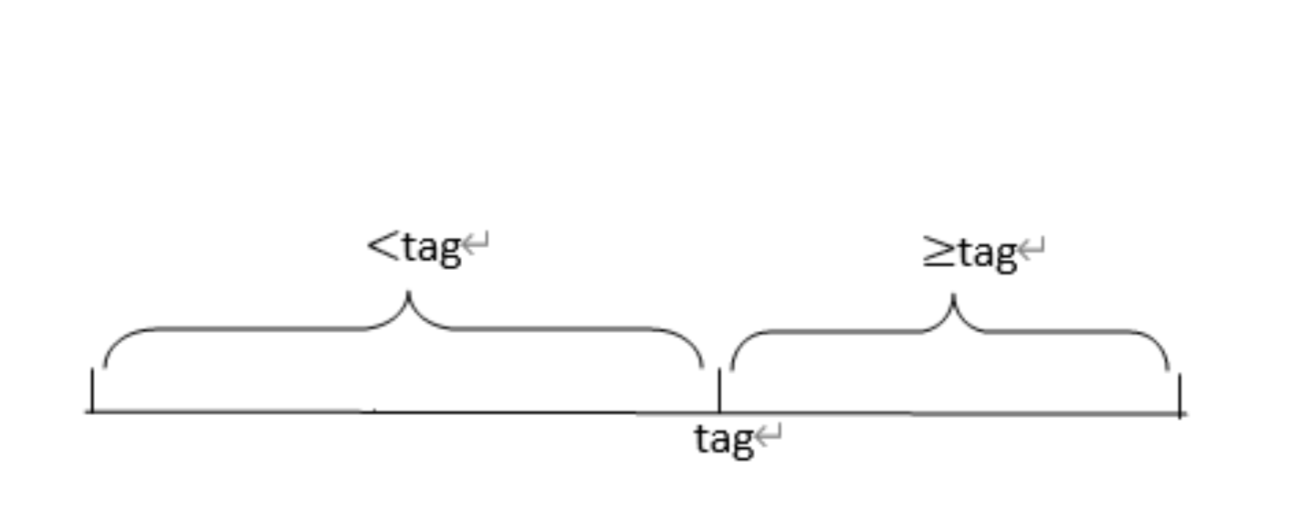
\includegraphics[width=10cm,height=3.5cm]{image/kth1.png}
		\caption{模仿快速排序}
	\end{minipage}
\end{figure}
这样我们得到了两个小一点的序列。为了后文的叙述方便,我们称在  t a g  左 侧的序列为  $N_{l}$,  长度为  $\left|N_{l}\right|$,  在$ \operatorname{tag}$ 右侧的序列为 $N_{r}$,  长度为$  \left|N_{r}\right|$ 。
到这一步,我们将问题拆解为如下三种情况:
$$
\text {question}(N, k)=\left\{\begin{aligned}
\text {question}\left(N_{l}, k\right) ,&\left|N_{l}\right|>=k \\
\text {tag} ,&\left|N_{l}\right|=k-1 \\
\text {question}\left(N_{r}, k-\left|N_{l}\right|-1\right) ,&\left|N_{l}\right|<k-1
\end{aligned}\right.
$$
按照上述方法不断递归下去,直到中间某一步达成 $ \left|N_{l}\right|=k-1$  的条件时, 就得到想要的结果了。
\section{复杂度分析}
因为算法中每一步的 tag都是随机取的,所以我们在分析复杂度时不仅要 考虑理想情况,也要考虑最坏情况。
最佳情况  \quad  每一次的  t a g  都恰好为序列的中间值,即每次操作都将问题规 模缩小为原来的一半。于是由经典的分治算法复杂度计算我们可以得到:
$$T(n)=T\left(\frac{n}{2}\right)+n$$
由主定理可以得到此时的时间复杂度
$$T(n) \in O(n)$$

最坏情况 每一次tag都恰好为序列的最大值或者最小值,即每次操作都 只能将问题规模减 1。于是我们可以的得到:
$$
T(n)=1+2+3+\cdots+(n-1)+n
$$
即
$$
T(n)=\frac{n(n+1)}{2}
$$
所以最坏情况的时间复杂度
$$
T(n) \in O\left(n^{2}\right)
$$
中间情况  \quad  我们虽然很难保证每次  t a g  的选取都恰好选中序列的中间值,但
如果我们能保证每次选取的  t a g  都在某个区间范围内,这种中间情况会比 最坏情况好很多。
比如,假如我们能够保证每次操作得到的  
$$\left|N_{l}\right|  $$
都满足式:

$$\frac{1}{4}|N| \leq\left|N_{l}\right| \leq \frac{3}{4}|N|$$


\input{src/dynamic-programming-1.tex}
\input{src/LN16.tex}
\input{src/Ln17-DP-ShortestPath.tex}
\input{src/LN18-DP-ZeroOneKnapsack.tex}
\input{src/Ln19-DP-ContextFreeGrammar.tex}
\input{src/network-flow-base.tex}
\input{src/Network-flows.tex}
\input{src/Image-segmentation.tex}
\input{src/Ln26-P-NP.tex}
\input{src/Proof-of-Statute.tex}
\input{src/Ln15-ApproximationAlgorithm.tex}


\bibliography{ref.bib}
\end{document}
